\section{Auswertung}
\label{sec:Auswertung}

\subsection{Bestimmung des spezifischen Widerstandes}
Die Dicke des Kupferdrahtes ist $d_{DK}=\qty{0.104(0.001)}{\milli\meter}$ und die des Silberdrahtes ist $d_{DS}=\qty{0.263()}{\milli\meter}$.
Mit 
\begin{equation}
  A=\pi \bigl(\frac{d}{2} \bigr)^2
\label{eqn:Querschnitt}
\end{equation}
\noindent 
kann dann die Fläche $A_{DK}=\qty{0.00849(0.00016)}{\milli\meter\squared}$ und $A_{DS}=\qty{0.0543(0.0004)}{\milli\meter\squared}$.
Für die Kupferspule, bei der die Länge des Drahtes $L_K=\qty{1.37}{\meter}$ ist, und für die Silberspule mit $L_S=\qty{1.73}{\meter}$, wird außerdem der ohmsche Widerstand gemessen.
Dieser beträgt $R_K=\qty{2.7050}{\ohm}$ und $R_S=\qty{0.6086}{\ohm}$.

Jetzt kann mit der Formel \ref{eqn:} der spezifische Widerstand von Kupfer und Silber bestimmt werden.


Für Kupfer beträgt dieser $\varrho_K=\qty{0.01677(0.00032)}{\ohm\milli\meter\squared\per\m}$ und für Silber $\varrho_S=\qty{0.00299(0.00006)}{\ohm\milli\meter\squared\per\m}$.

Bei Zink ist der spezifische Widerstand $\varrho_Z = \qty{0.06}{\ohm\milli\meter\squared\per\m}$ \cite{Zink}.

\begin{figure}
  \centering
  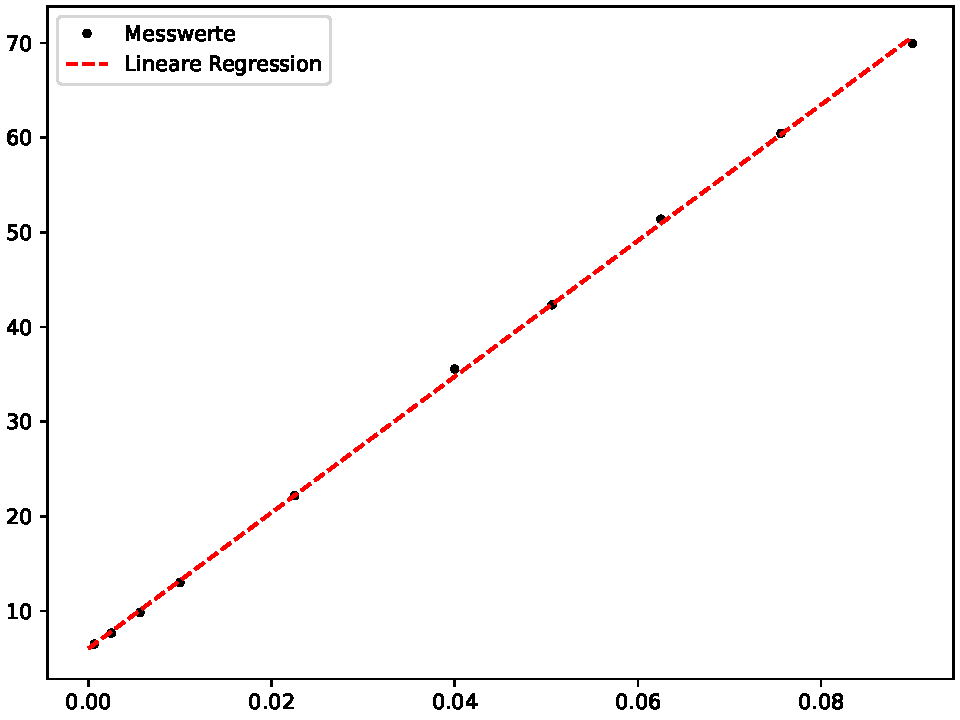
\includegraphics{plot.pdf}
  \caption{Plot.}
  \label{fig:plot}
\end{figure}

\begin{table}
  \centering
  \caption{Eine Beispieltabelle mit Messdaten.}
  \label{tab:tabelle}
  \sisetup{table-format=1.1, per-mode=reciprocal}
  \begin{tblr}{
      colspec = {S[table-format=3.0] S[table-format=2.1] S},
      row{1} = {guard, mode=math},
      vline{4} = {2}{-}{text=\clap{$\pm$}},
    }
    \toprule
    U \mathbin{/} \unit{\volt} & I \mathbin{/} \unit{\micro\ampere} & \SetCell[c=2]{c} N \mathbin{/} \unit{\per\second} & \\
    \midrule
    360 & 0.1 & 98.3 & 0.9 \\
    400 & 0.2 & 99.8 & 1.0 \\
    420 & 0.2 & 99.1 & 0.9 \\
    \bottomrule
  \end{tblr}
\end{table}

Siehe \autoref{fig:plot} und \autoref{tab:tabelle}!
